\documentclass[a4paper, 11pt]{article}
\usepackage[francais]{babel}
\usepackage[utf8]{inputenc}
\usepackage[T1]{fontenc}
\usepackage{float}
\usepackage{graphicx}
\usepackage{datetime}
\usepackage{comment} % enables the use of multi-line comments (\ifx \fi)

\usepackage{fullpage} % changes the margin

\begin{document}
%Header-Make sure you update this information!!!!
\noindent
\large\textbf{\'Etude Comparative 1} \hfill \textbf{Distribution de l'eau en Haïti} \\
\normalsize Deknop Céline \hfill Université Catholique de Louvain \\
Hallet Adrien \hfill \today \\
Strebelle Sébastien

\section*{Abstract}
\'Evaluer les usages et offres, en termes de systèmes d'information et de communication, dans le domaine de la gestion de distribution d'eau potable.

\hrule
\section*{Termes}
\begin{description}
    \item[GIS] Geographic Information System. Terme général désignant des logiciels ayant au moins une composante d'information géographique, souvent accompagnée de visuels.
    \item[CAD] Computer Assisted Design. En Français DAO pour Dessin Assisté par Ordinateur.
\end{description}
\section*{Sujets d'étude}
Afin de pouvoir comparer l'offre existante, les solutions existantes ayant été analysées sont :
\begin{description}
    \item[EPANET 2] Développé par la \textit{United States Environment Protection Agency}, qui a notamment pour charge la gestion de ressources acqueuses aux \'Etats-Unis d'Amérique. Le logiciel est libre de droits et un toolkit open-source avec une API en C. L'API rend ce programme à la base de nombreux autres logiciels de gestion. Référencé à de nombreuses reprises dans les documentations d'autres outils, EPANET est un système de référence en la matière.
    \item[WaterGEMS / WaterCAD] Développé par Bentley, le logiciel s'inspire de suites bureautiques logicielles connues pour offrir une interface plus moderne à l'utilisateur et des visuels avancés.
    \item[Innovyze InfoWater] Construit sur la plateforme ArcGIS (logiciel d'analyse géographique)
    \item[KY Pipe] Construit sur EPANET, le logiciel est issu de l'université du Kentucky et se concentre sur l'analyse hydraulique. Son ancienneté de 40 ans en fait l'un des plus utilisés au monde, notamment par sa capacité à modélier de nombreux contenus (eau, pétrole, composants chimiques, etc)
    \item[HydrauliCAD] Basé sur AutoCAD (logiciel de dessin assisté par ordinateur le plus répandu dans le monde selon Forbes\footnote{www.forbes.com/sites/zacks/2013/09/06/autodesk-is-no-blueprint-for-gains})
\end{description}
Il est à noter que de nombreux logiciels existent pour modéliser et analyser les réseaux de distribution, mais il est inutile de tous les analyser car la plupart énoncent dans leurs crédits et/ou manuels se baser sur des toolkits identiques, principalement EPANET et AutoCAD.

\section{Similarités}
Dans cette section, nous énonçons les similarités relevées entre les logiciels
\subsection{Séparation modulaire}
On remarque le retour systématique, propre à de nombreux logiciels de gestion par modèle (PetriNET, etc), de trois modules.
\begin{description}
    \item[Modélisation graphique] L'utilisateur se sert d'outils prédéfinis pour modéliser le réseau de manière graphique et/ou géographique (insertion des coordonnées GPS).
    \item[Analyse formelle] L'utilisateur peut choisir des modèles mathématiques à appliquer aux données et ainsi évaluer le système sur les critères de son choix (performances, qualité, ...)
    \item[Rapports d'état] L'utilisateur peut consulter des rapports accompagnés d'informations graphiques
\end{description}

\subsection{Affichage du réseau}
Tous les logiciels présentent le réseau de distribution sous forme d'un graphe où les liens représentes des conduites d'acheminement (tuyeaux, canaux, etc) et les noeuds sont des points de traitement/rétention (bassins, stations, branchements, sondes, etc)

\begin{minipage}{\linewidth}
      \centering
      \begin{minipage}{0.45\linewidth}
          \begin{figure}[H]
              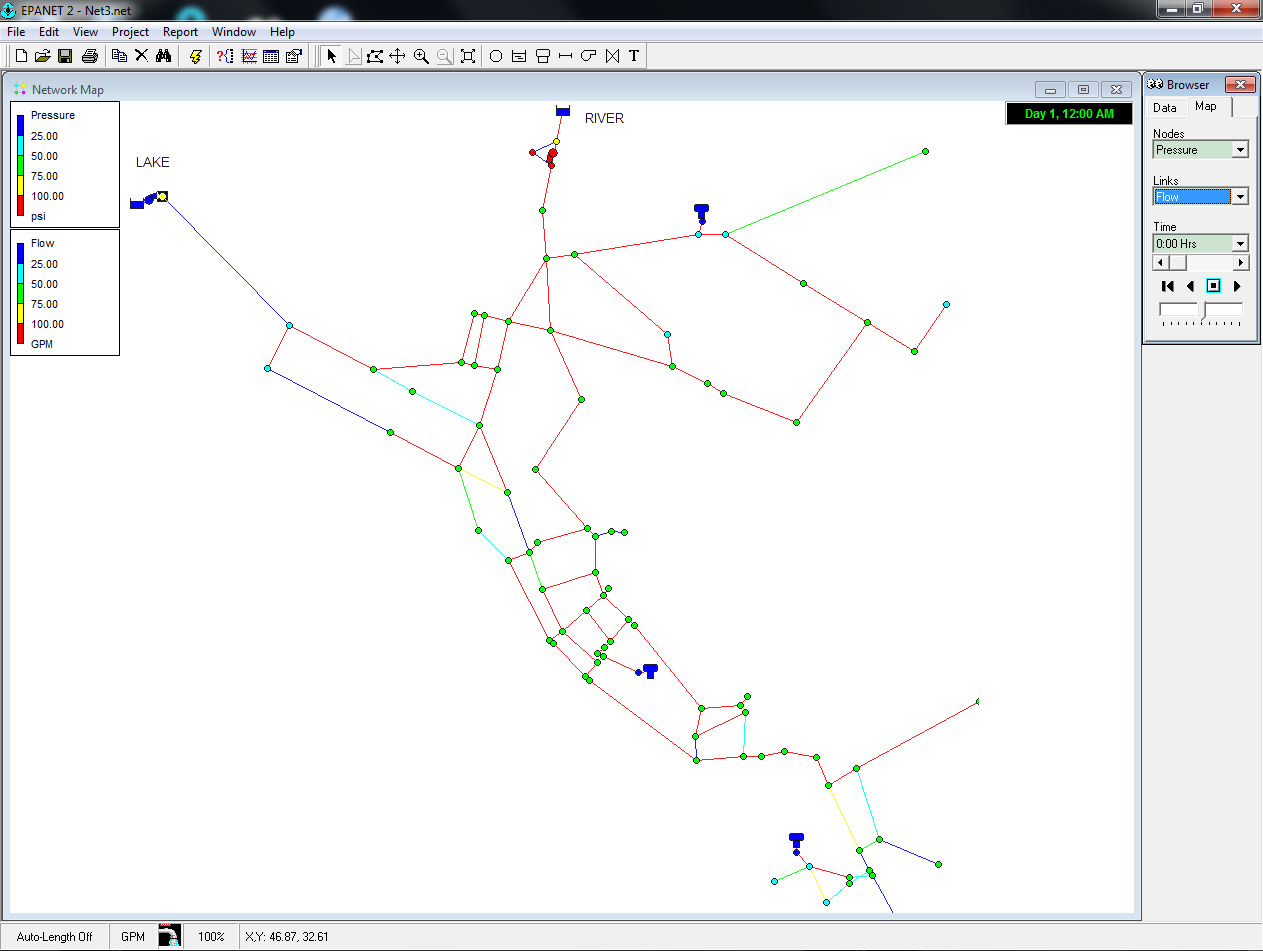
\includegraphics[width=\linewidth]{Etude_Comparative_1/epanet}
              \caption{Réseau dans EPANet}
          \end{figure}
      \end{minipage}
      \hspace{0.05\linewidth}
      \begin{minipage}{0.45\linewidth}
          \begin{figure}[H]
              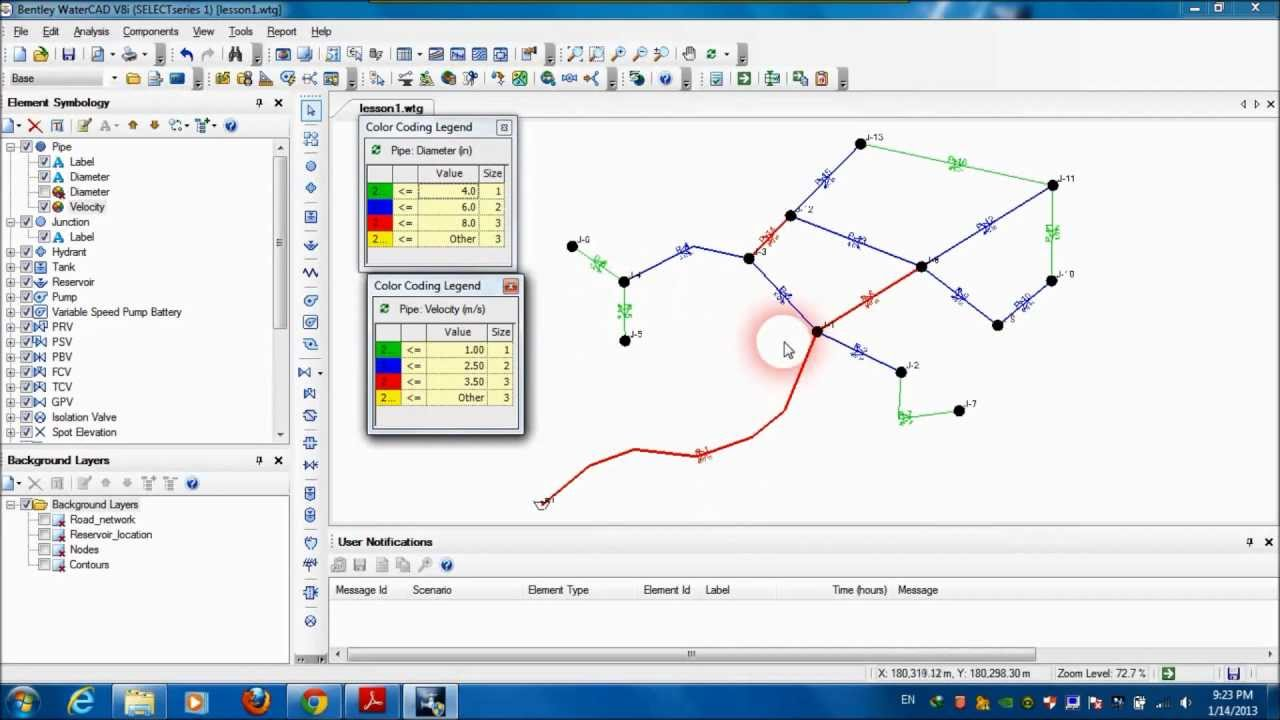
\includegraphics[width=\linewidth]{Etude_Comparative_1/watercad}
              \caption{Réseau dans WaterCAD}
          \end{figure}
      \end{minipage}
  \end{minipage}

\begin{minipage}{\linewidth}
      \centering
      \begin{minipage}{0.45\linewidth}
          \begin{figure}[H]
              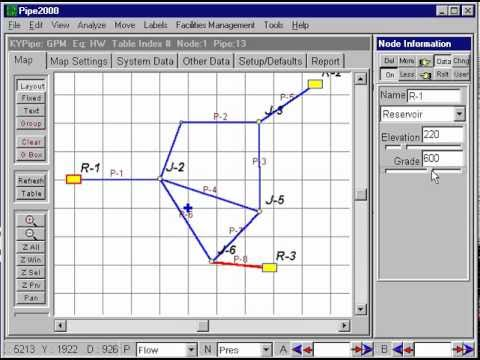
\includegraphics[width=\linewidth]{Etude_Comparative_1/kypipe}
              \caption{Réseau dans KY Pipe}
          \end{figure}
      \end{minipage}
      \hspace{0.05\linewidth}
      \begin{minipage}{0.45\linewidth}
          \begin{figure}[H]
              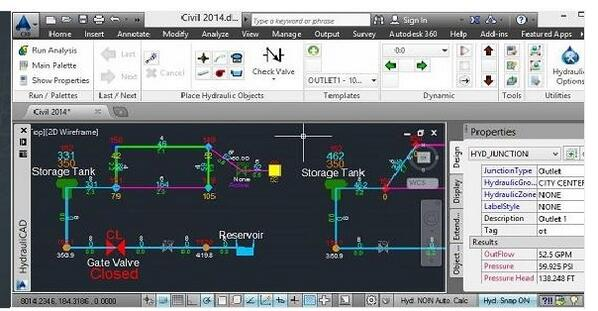
\includegraphics[width=\linewidth]{Etude_Comparative_1/hydraulicad}
              \caption{Réseau dans HydrauliCAD}
          \end{figure}
      \end{minipage}
  \end{minipage}

\newpage
\subsection{Superposition du réseau}
La très large majorité des logiciels exploite la possibilité de superposer le graphe du réseau à des plans ou vues satellitaires. Certains logiciels utilisent des fonctions d'export vers des logiciels de cartographies, il y a également des solutions utilisant des outils de cartographie plus connus (e.g.: Google Maps) intégrés dans le logiciel. Enfin, d'autres proposent d'importer des plans et d'ajuster leur échelle au réseau modélisé.

\begin{minipage}{\linewidth}
      \centering
      \begin{minipage}{0.45\linewidth}
          \begin{figure}[H]
              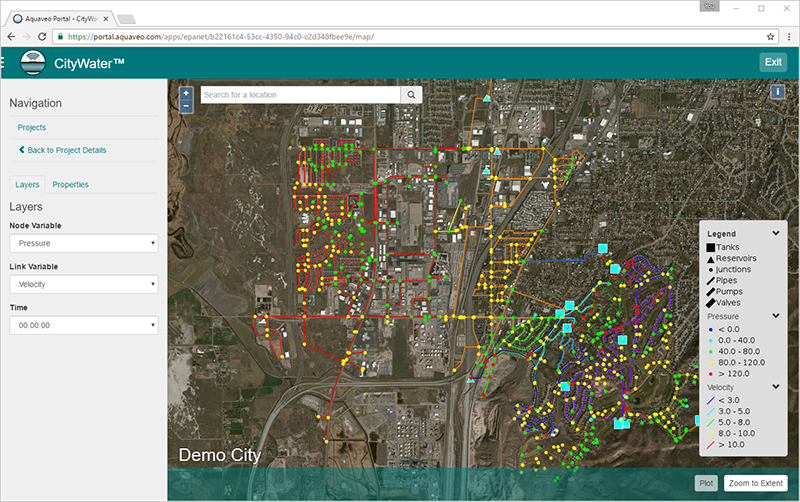
\includegraphics[width=\linewidth]{Etude_Comparative_1/citywater}
              \caption{CityWater basé sur EPANet}
          \end{figure}
      \end{minipage}
      \hspace{0.05\linewidth}
      \begin{minipage}{0.45\linewidth}
          \begin{figure}[H]
              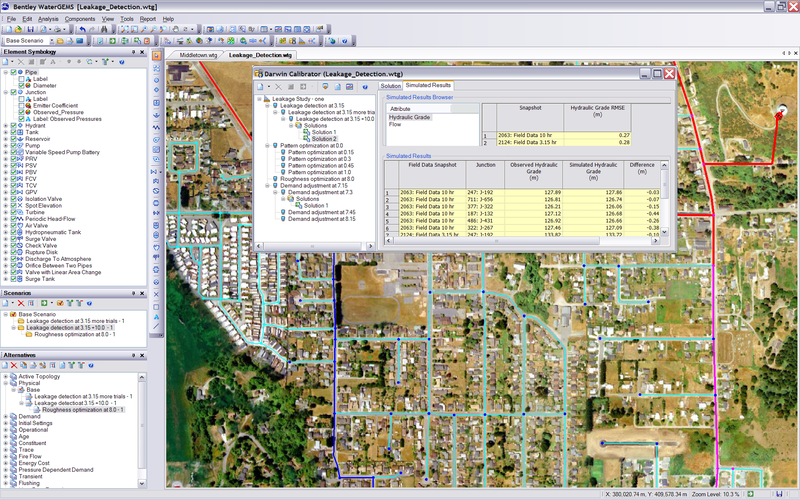
\includegraphics[width=\linewidth]{Etude_Comparative_1/watergems}
              \caption{Plan dans WaterCAD}
          \end{figure}
      \end{minipage}
  \end{minipage}

\begin{minipage}{\linewidth}
      \centering
      \begin{minipage}{0.45\linewidth}
          \begin{figure}[H]
              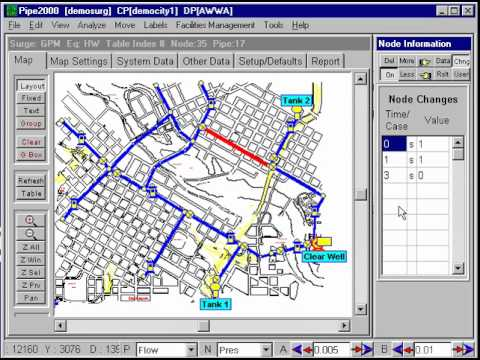
\includegraphics[width=\linewidth]{Etude_Comparative_1/kypipeplan}
              \caption{Plan dans KY Pipe}
          \end{figure}
      \end{minipage}
      \hspace{0.05\linewidth}
      \begin{minipage}{0.45\linewidth}
          \begin{figure}[H]
              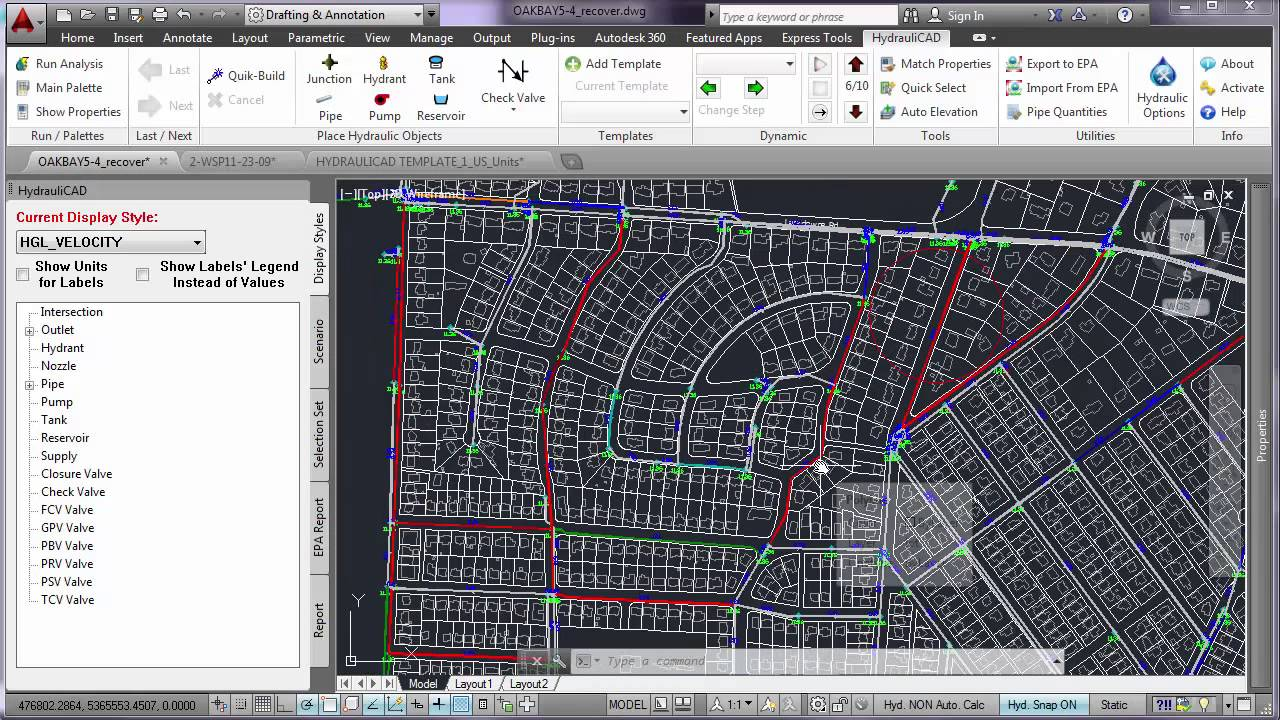
\includegraphics[width=\linewidth]{Etude_Comparative_1/hydraulicadplan}
              \caption{Plan dans HydrauliCAD}
          \end{figure}
      \end{minipage}
  \end{minipage}

\subsection{Analyses détaillées et graphiques}
La totalité des logiciels étudiés offrent des possibilités d'analyse mathématiques spécifiques telles les études de :
\begin{itemize}
    \item Flux en un point / segment
    \item Dépôt en un point / segment
    \item Calculs de pression
    \item ...
\end{itemize}
Ainsi que des modélisations à plus grande échelle sur tout le réseau ou une partie de celui-ci, par exemple :
\begin{itemize}
    \item Flux total transporté
    \item Distance couverte sur une période de temps donné
    \item Temps de renouvellement du réseau
    \item ...
\end{itemize}

Notons que les analyses générales se consultent généralement par le biais de \textbf{menus spécifiques} tandis que les analyses en un point sont généralement associées (au moins partiellement) au \textbf{clic sur le noeud associé dans le graphe}.

Il est également important de noter que, comme énoncé ci-avant, les outils mathématiques utilisés dans le cadre de ces études sont majoritairement importées, la bibliothèque la plus utilisée étant celle d'EPANET, référencée par près de 40\% des logiciels étudiés (y compris KY Pipe, HydrauliCAD, WaterGEMS, InfoWater)

\section{Dissemblances}
Dans cette section nous étudions les différences principales établies entre les logiciels étudiés. En excluant les choix mineurs d'agencement et de fonctionnement des outils, il y n'y a que peu ou pas de différences fonctionnelles entre les logiciels. Les dissemblances marquantes sont principalement :

\begin{description}
    \item[Tarifaires] La gamme des prix varie énormément. EPANET est libre et open-source et donc gratuit tandis qu'à l'autre extrême, la licence complète d'InfoWater coûter 14.000\$. Plusieurs des logiciels payants proposent des plans tarifaires à échelons où les différentes versions proposent des limites différentes sur la quantités de composants (tuyaux, noeuds, ...) du réseau.
    \item[Visuelles] EPANET est une solution gratuite et propose une interface rudimentaire monochrome tandis que les solutions payantes proposées par de plus grosses productions (e.g.: WaterGEMS) avancent des interfaces plus intuitives et accueillantes ainsi que des rapports et graphiques plus modernes dont la qualité permet l'intégration directe à des documents et publications.
\end{description}

\section*{Conclusion}
Il existe peu de différences entre les logiciels. Les fonctionnalités sont identiques et seul l'avancement de celles-ci diffère en fonction du plan tarifaire.

Nous avons également pu remarquer que la plupart des outils majeurs se basaient sur les mêmes bibliothèques. Nous avons donc pu relever l'importance d'EPANET et de sa bibliothèque mathématique\footnote{Bibliothèque implémentée en C, EPANET 2 est une version standalone permettant d'utiliser les outils visuels du logiciel} qui est l'une des plus utilisées.

Enfin, nous relevons l'importance du système d'interface par graphe permettant la visualisation du réseau et l'interaction avec celui-ci, qu'il soit ou non superposé à des images satellitaires, cartes, plans cadastraux.
\end{document}
